\documentclass[aspectratio=169]{beamer}

\usetheme{Madrid}
\usecolortheme{seahorse}

\usepackage{graphicx}
\usepackage{booktabs}
\usepackage{hyperref}
\usepackage{tikz}
\usetikzlibrary{calc}
\usepackage{xcolor}
\usepackage{amssymb}

% Custom colours
\definecolor{accentblue}{RGB}{0, 90, 156}
\definecolor{lightgray}{RGB}{240, 240, 240}
\definecolor{darkgray}{RGB}{80, 80, 80}
\definecolor{warnred}{RGB}{192, 0, 0}
\definecolor{okgreen}{RGB}{0, 130, 80}

\setbeamercolor{frametitle}{bg=accentblue, fg=white}

\setbeamercolor{titlelike}{parent=structure}
\setbeamercolor{palette primary}{bg=accentblue}
\setbeamercolor{palette secondary}{bg=accentblue!80}
\setbeamercolor{palette tertiary}{bg=accentblue!60}

\setbeamertemplate{navigation symbols}{}
\setbeamertemplate{itemize items}[circle]

% Dashed image placeholder: \imgph{width}{height}{caption}
\newcommand{\imgph}[3][4.5cm]{%
  \begin{tikzpicture}
    \node[
        draw=accentblue!40,
        dashed,
        rounded corners=4pt,
        fill=lightgray,
        inner sep=8pt,
        minimum width=#1,
        minimum height=#2,
        align=center,
        text width={$(#1)-0.35cm$}
    ]{\footnotesize\textbf{[Image]}\\[2pt]\scriptsize #3};
  \end{tikzpicture}
}

% ---------- metadata ----------
\title{Road Injury Hospitalisation Analysis}
\subtitle{Progress Report --- Design Book \& D3 Charts}
\author{Duc Thanh \& Douglas Luong \\ \small CL01/T08 / COS30045}
\date{\today}

% ==============================
\begin{document}

% ---- Title slide ----
\begin{frame}
  \titlepage
\end{frame}

% ---- Agenda ----
\begin{frame}{Overview}
  \tableofcontents
\end{frame}

% ==============================
\section{Data \& Pipeline}

\begin{frame}{Dataset \& Data Source}
  \begin{columns}[T]
    \begin{column}{0.55\textwidth}
      \textbf{Primary dataset}
      \begin{itemize}
        \item \texttt{transformed\_datasets.xlsx}\\
              {\small Sheets: \texttt{publication}, \texttt{state}, \texttt{state\_summary}, \texttt{population}, \ldots}
        \item National road crash hospitalisations (BITRE)
        \item Examined period: \textbf{2011 -- 2021}
      \end{itemize}
      \vspace{0.4em}
      \textbf{Data pipeline (planned)}
      \begin{itemize}
        \item One JavaScript loader opens \texttt{transformed\_datasets.xlsx}
        \item Each sheet parsed to in-memory CSV-style tables
        \item Loader calls chart init functions (\texttt{initCh1}--\texttt{initCh4})
        \item \textbf{No JSON} --- charts read sheet data directly
        \item GeoJSON kept for map geometry only (\texttt{au-states.geojson})
      \end{itemize}
    \end{column}
    \begin{column}{0.42\textwidth}
      \imgph{4.8cm}{3.2cm}{Pipeline: xlsx $\to$ JS loader $\to$ chart modules}
      \vspace{0.4em}
      \begin{block}{\footnotesize Source}
        \footnotesize BITRE hospitalised-injury publications
      \end{block}
    \end{column}
  \end{columns}
\end{frame}

% ==============================
\section{Current Web Version}

\begin{frame}{Design Book --- Live Site}
  \begin{columns}[T]
    \begin{column}{0.52\textwidth}
      \textbf{Stack \& deployment}
      \begin{itemize}
        \item Vanilla JS + \textbf{Vite}; charts in \textbf{D3}
        \item Scrollytelling: 5 chapters, sticky chart panels
        \item Mercury: \url{https://mercury.swin.edu.au/cos30045/s104358130/design-book/}
      \end{itemize}
      \vspace{0.35em}
      \textbf{Story arc}
      \begin{enumerate}
        \item National picture \quad \texttt{\#chapter-1}
        \item Where (states) \quad \texttt{\#chapter-2}
        \item Who (demographics) \quad \texttt{\#chapter-3}
        \item How (road user) \quad \texttt{\#chapter-4}
        \item Convergence \quad \texttt{\#chapter-5}
      \end{enumerate}
    \end{column}
    \begin{column}{0.44\textwidth}
      \imgph{4.8cm}{4.2cm}{Homepage: header, chapter nav, hero copy}
    \end{column}
  \end{columns}
\end{frame}

\begin{frame}{Implementation Status}
  \begin{columns}[T]
    \begin{column}{0.50\textwidth}
      \textbf{Completed (prototype)}
      \begin{itemize}
        \item[\textcolor{okgreen}{\checkmark}] HTML narrative + scrolly steps per chapter
        \item[\textcolor{okgreen}{\checkmark}] Dark-mode CSS tokens; charts inherit palette
        \item[\textcolor{okgreen}{\checkmark}] Charts 1--4 D3 modules in \texttt{.placeholder-canvas}
        \item[\textcolor{okgreen}{\checkmark}] \texttt{main.js}: scrolly first; chart inits isolated via \texttt{.catch()}
      \end{itemize}
      {\footnotesize\textcolor{darkgray}{Prototype loads \texttt{*.json}; target is xlsx $\to$ CSV in one JS file.}}
      \vspace{0.35em}
      \textbf{In progress / planned}
      \begin{itemize}
        \item[\textcolor{warnred}{[!]}] Single JS xlsx $\to$ CSV loader (replace JSON fetch path)
        \item[\textcolor{warnred}{[!]}] Chapter 5 heatmap (\texttt{\#chart-5-heatmap}) --- placeholder only
        \item[\textcolor{warnred}{[!]}] Chart 2: choropleth hue (replacing sized bubbles)
        \item[\textcolor{warnred}{[!]}] \texttt{stepchange} listeners (phase reveal, drill spotlight)
      \end{itemize}
    \end{column}
    \begin{column}{0.46\textwidth}
      \imgph{5cm}{3.6cm}{Full-page scroll: one chapter sticky panel + step text}
      \vspace{0.3em}
      {\footnotesize\textcolor{darkgray}{Modules: \texttt{ch1-trend}, \texttt{ch2-states}, \texttt{ch3-demographics}, \texttt{ch4-roaduser}, shared \texttt{theme.js}}}
    \end{column}
  \end{columns}
\end{frame}

% ==============================
\section{Final Chart Design}

\begin{frame}{Chart 1 --- National Trend (Line)}
  \begin{columns}[T]
    \begin{column}{0.50\textwidth}
      \textbf{Spec} (\texttt{publication} sheet)
      \begin{itemize}
        \item Line: year (x) vs hospitalisation count (y)
        \item Background: dotted light-gray grid
        \item \textbf{Admission} column built in \textbf{JavaScript} on first load (same DAX rule):
        \begin{itemize}
          \item 2011: ``Hospitalised injuries''
          \item 2012--2016: ``Change in admissions 2012''
          \item 2017+: ``Change in admissions 2017''
        \end{itemize}
        \item Hover at year $\to$ tooltip: year + case count
      \end{itemize}
      \vspace{0.2em}
      {\footnotesize Data: \texttt{publication} sheet $\to$ CSV rows; no \texttt{.json} file}
    \end{column}
    \begin{column}{0.46\textwidth}
      \imgph{5cm}{3.5cm}{Chart 1 screenshot (\texttt{\#chart-1-trend})}
    \end{column}
  \end{columns}
\end{frame}

\begin{frame}{Chart 2 --- States (Map + Drill)}
  \begin{columns}[T]
    \begin{column}{0.50\textwidth}
      \textbf{Map layer} (\texttt{state} / \texttt{state\_summary})
      \begin{itemize}
        \item Australia polygons filled with \textbf{one accent hue}
        \item \textbf{No sized bubbles} --- raw totals mislead when populations differ
        \item Hue intensity encodes comparable burden (e.g.\ rate or normalised metric)
        \item Hover: state label + value + ``click to see more''
        \item Click $\to$ drill: line (cases) + bar (population)
      \end{itemize}
      \textbf{Drill notes}
      \begin{itemize}
        \item Back button top-left
        \item \textbf{VIC}: admission change from 2012 (segment legend)
        \item \textbf{NSW}: admission change from 2017
      \end{itemize}
    \end{column}
    \begin{column}{0.46\textwidth}
      \imgph{5cm}{3.2cm}{Choropleth map (\texttt{\#chart-2-states})}\\[0.2em]
      \imgph{5cm}{1.6cm}{Drill: line $\times$ bar for one state}
    \end{column}
  \end{columns}
\end{frame}

\begin{frame}{Charts 3 \& 4 --- Demographics \& Road User}
  \begin{columns}[T]
    \begin{column}{0.48\textwidth}
      \textbf{Chart 3 --- Clustered horizontal bars}
      \begin{itemize}
        \item \texttt{publication} sheet $\to$ CSV rows (age $\times$ sex)
        \item Small multiples by age band; filter: gender
        \item Bars: cases vs bed days; labels at bar ends
        \item Vertical dotted grid; drop missing age groups in JS
        \item Pills: All / Female / Male (morph on change)
      \end{itemize}
      \vspace{0.35em}
      \imgph{4.6cm}{2.2cm}{Chart 3 (\texttt{\#chart-3-demographics})}
    \end{column}
    \begin{column}{0.48\textwidth}
      \textbf{Chart 4 --- Dumbbell}
      \begin{itemize}
        \item \texttt{publication} sheet $\to$ CSV rows (road user)
        \item y = road user; x: cases vs bed days on shared scale
        \item Dotted grid; legend top-left
        \item Hover row $\to$ user, cases, bed days, ratio
        \item Exclude ``Not applicable'' when loading data
      \end{itemize}
      \vspace{0.35em}
      \imgph{4.6cm}{2.2cm}{Chart 4 (\texttt{\#chart-4-mechanism})}
    \end{column}
  \end{columns}
\end{frame}

\begin{frame}{Chart 5 --- Convergence (Pending)}
  \begin{columns}[T]
    \begin{column}{0.55\textwidth}
      \textbf{Planned}
      \begin{itemize}
        \item Heatmap / matrix: states $\times$ road users
        \item Highlights highest-burden profile in narrative copy
        \item Placeholder canvas retained in \texttt{index.html}
      \end{itemize}
      \vspace{0.5em}
      \begin{alertblock}{Design alignment}
        Final chart types move beyond bar/line-only Power BI drafts; map, small multiples, and dumbbell match the approved spec.
      \end{alertblock}
    \end{column}
    \begin{column}{0.42\textwidth}
      \imgph{4.8cm}{3.8cm}{Chart 5 wireframe (\texttt{\#chart-5-heatmap})}
    \end{column}
  \end{columns}
\end{frame}

% ==============================
\section{D3 Coding Plan}

\begin{frame}{Architecture Overview}
  \begin{columns}[T]
    \begin{column}{0.52\textwidth}
      \textbf{Loader --- single JavaScript entry}
      \begin{itemize}
        \item Open \texttt{transformed\_datasets.xlsx} (e.g.\ SheetJS)
        \item Parse each sheet to CSV-style row arrays
        \item Shared filters: missing ages, ``Not applicable'' road users
        \item Derive \texttt{admission} column in JS (Chart 1; VIC/NSW drill)
        \item Call \texttt{initCh1}--\texttt{initCh4} with table arguments
      \end{itemize}
      \textbf{Shared --- \texttt{src/charts/theme.js}}
      \begin{itemize}
        \item \texttt{phasePalette}, \texttt{fmt}, \texttt{mountSvg}, \texttt{drawGrid}, \texttt{makeTooltip}
      \end{itemize}
      \vspace{0.2em}
      \textbf{Run} --- \texttt{npm run dev} / \texttt{npm run build}
    \end{column}
    \begin{column}{0.44\textwidth}
      \begin{tikzpicture}[font=\footnotesize, every node/.style={align=center}]
        \node[draw=accentblue, rounded corners, fill=lightgray, inner sep=6pt, text width=4.2cm] (xlsx) {transformed\_datasets.xlsx};
        \node[draw=accentblue, rounded corners, fill=lightgray, inner sep=6pt, text width=4.2cm, below=0.45cm of xlsx] (js) {data loader (JS)};
        \node[draw=accentblue, rounded corners, fill=lightgray, inner sep=6pt, text width=4.2cm, below=0.45cm of js] (csv) {sheets $\to$ CSV tables};
        \node[draw=accentblue, rounded corners, fill=lightgray, inner sep=6pt, text width=4.2cm, below=0.45cm of csv] (d3) {ch1--ch4 + theme.js};
        \draw[->, accentblue, thick] (xlsx) -- (js);
        \draw[->, accentblue, thick] (js) -- (csv);
        \draw[->, accentblue, thick] (csv) -- (d3);
      \end{tikzpicture}
      \vspace{0.4em}
      {\footnotesize\textcolor{darkgray}{No \texttt{public/data/*.json}; GeoJSON only for map outlines}}
    \end{column}
  \end{columns}
\end{frame}

\begin{frame}{Scrolly Integration (Follow-up)}
  \begin{itemize}
    \item \texttt{IntersectionObserver} + \texttt{stepchange} \texttt{CustomEvent} already drive sticky panels
    \item Charts render \textbf{once on load}; they do not yet subscribe to steps
    \item Planned hooks per chapter, e.g.:
    \begin{itemize}
      \item Ch.\,1: phase reveal along national line
      \item Ch.\,2: choropleth highlight before drill
      \item Ch.\,4: view morph between metrics
    \end{itemize}
  \end{itemize}
  \vspace{0.5em}
\end{frame}

% ==============================
\section{Blockers \& Challenges}

\begin{frame}{Blockers \& Challenges}
  \begin{block}{[!]\quad Challenge 1 --- Comparable State Burden}
    Raw hospitalisation totals \textbf{cannot be compared across states} (population size).\\
    \smallskip
    \textit{Response:} replace centroid bubbles with a \textbf{single-hue choropleth}; encode a normalised or rate-based metric on fill. Drill view still shows raw cases + population bars for context.
  \end{block}

  \vspace{0.4em}

  \begin{block}{[Chart]\quad Challenge 2 --- Chapter 5 Not Implemented}
    Convergence matrix design and data join still open; narrative in HTML is ahead of the viz.
  \end{block}

  \vspace{0.4em}

  \begin{alertblock}{[!]\quad Challenge 3 --- Pipeline Migration}
    Prototype still fetches \texttt{*.json}; refactor to xlsx-in-browser loader and retire \texttt{build\_data.py}.
  \end{alertblock}
\end{frame}

% ==============================
\section{Next Steps}

\begin{frame}{Next Steps}
  \begin{columns}[T]
    \begin{column}{0.50\textwidth}
      \begin{enumerate}
        \setlength\itemsep{0.45em}
        \item \textbf{Implement JS xlsx loader}\\
              {\small One file: open xlsx, sheets $\to$ CSV, call chart inits}
        \item \textbf{Refactor Chart 2 to choropleth hue}\\
              {\small Drop bubble sizing; normalise for fair state comparison}
        \item \textbf{Admission column in JS}\\
              {\small Chart 1 + VIC/NSW drill segments on first load}
        \item \textbf{Implement Chart 5 heatmap}\\
              {\small State $\times$ road-user matrix; wire \texttt{\#chart-5-heatmap}}
        \item \textbf{Connect \texttt{stepchange} to charts 1--4}\\
              {\small Scroll-driven highlights and transitions}
        \item \textbf{Capture screenshots for report \& slides}\\
              {\small Replace \texttt{[Image]} placeholders in \texttt{IMAGES/}}
        \item \textbf{Finalise written report}\\
              {\small Deadline: 11/06/2026}
        \item \textbf{KNIME migration / validation}\\
              {\small Satisfy submission requirements alongside pbix}
      \end{enumerate}
    \end{column}
    \begin{column}{0.46\textwidth}
      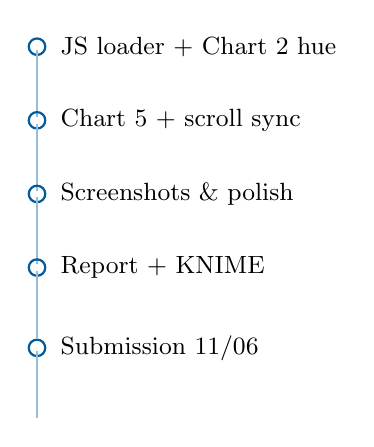
\begin{tikzpicture}[scale=0.85, every node/.style={font=\small}]
        \foreach \y/\label in {
          4.5/{JS loader + Chart 2 hue},
          3.4/{Chart 5 + scroll sync},
          2.3/{Screenshots \& polish},
          1.2/{Report + KNIME},
          0.0/{Submission 11/06}
        }{
          \draw[accentblue, thick] (0,\y) circle (3.5pt);
          \draw[accentblue!40, thick] (0,\y-0.05) -- (0,\y-1.05);
          \node[right=5pt] at (0,\y) {\label};
        }
      \end{tikzpicture}
      \vspace{0.5em}
    \end{column}
  \end{columns}
\end{frame}

% ---- Closing ----
\begin{frame}[plain]
  \begin{center}
    \vspace{1.5cm}
    {\Large \textbf{Thank you}}\\[0.8em]
    {\normalsize Questions welcome}\\[1.5em]
    \textcolor{darkgray}{\small Duc Thanh x Douglas Luong \quad|\quad 105548505@student.swin.edu.au \quad|\quad \today}\\[0.6em]
    {\footnotesize\url{https://mercury.swin.edu.au/cos30045/s104358130/design-book/}}
  \end{center}
\end{frame}

\end{document}